% Created by tikzDevice version 0.12.4 on 2023-06-03 16:04:13
% !TEX encoding = UTF-8 Unicode
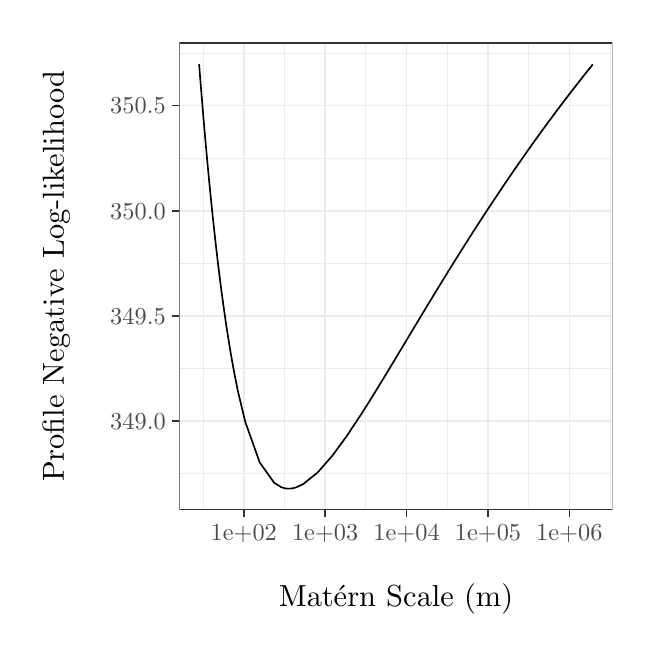
\begin{tikzpicture}[x=1pt,y=1pt]
\definecolor{fillColor}{RGB}{255,255,255}
\path[use as bounding box,fill=fillColor,fill opacity=0.00] (0,0) rectangle (216.81,216.81);
\begin{scope}
\path[clip] (  0.00,  0.00) rectangle (216.81,216.81);
\definecolor{drawColor}{RGB}{255,255,255}
\definecolor{fillColor}{RGB}{255,255,255}

\path[draw=drawColor,line width= 0.6pt,line join=round,line cap=round,fill=fillColor] (  0.00,  0.00) rectangle (216.81,216.81);
\end{scope}
\begin{scope}
\path[clip] ( 54.83, 42.57) rectangle (211.31,211.31);
\definecolor{fillColor}{RGB}{255,255,255}

\path[fill=fillColor] ( 54.83, 42.57) rectangle (211.31,211.31);
\definecolor{drawColor}{gray}{0.92}

\path[draw=drawColor,line width= 0.3pt,line join=round] ( 54.83, 55.69) --
	(211.31, 55.69);

\path[draw=drawColor,line width= 0.3pt,line join=round] ( 54.83, 93.69) --
	(211.31, 93.69);

\path[draw=drawColor,line width= 0.3pt,line join=round] ( 54.83,131.68) --
	(211.31,131.68);

\path[draw=drawColor,line width= 0.3pt,line join=round] ( 54.83,169.68) --
	(211.31,169.68);

\path[draw=drawColor,line width= 0.3pt,line join=round] ( 54.83,207.68) --
	(211.31,207.68);

\path[draw=drawColor,line width= 0.3pt,line join=round] ( 63.38, 42.57) --
	( 63.38,211.31);

\path[draw=drawColor,line width= 0.3pt,line join=round] ( 92.79, 42.57) --
	( 92.79,211.31);

\path[draw=drawColor,line width= 0.3pt,line join=round] (122.21, 42.57) --
	(122.21,211.31);

\path[draw=drawColor,line width= 0.3pt,line join=round] (151.62, 42.57) --
	(151.62,211.31);

\path[draw=drawColor,line width= 0.3pt,line join=round] (181.03, 42.57) --
	(181.03,211.31);

\path[draw=drawColor,line width= 0.3pt,line join=round] (210.45, 42.57) --
	(210.45,211.31);

\path[draw=drawColor,line width= 0.6pt,line join=round] ( 54.83, 74.69) --
	(211.31, 74.69);

\path[draw=drawColor,line width= 0.6pt,line join=round] ( 54.83,112.69) --
	(211.31,112.69);

\path[draw=drawColor,line width= 0.6pt,line join=round] ( 54.83,150.68) --
	(211.31,150.68);

\path[draw=drawColor,line width= 0.6pt,line join=round] ( 54.83,188.68) --
	(211.31,188.68);

\path[draw=drawColor,line width= 0.6pt,line join=round] ( 78.08, 42.57) --
	( 78.08,211.31);

\path[draw=drawColor,line width= 0.6pt,line join=round] (107.50, 42.57) --
	(107.50,211.31);

\path[draw=drawColor,line width= 0.6pt,line join=round] (136.91, 42.57) --
	(136.91,211.31);

\path[draw=drawColor,line width= 0.6pt,line join=round] (166.33, 42.57) --
	(166.33,211.31);

\path[draw=drawColor,line width= 0.6pt,line join=round] (195.74, 42.57) --
	(195.74,211.31);
\definecolor{drawColor}{RGB}{0,0,0}

\path[draw=drawColor,line width= 0.6pt,line join=round] ( 61.95,203.64) --
	( 62.27,199.44) --
	( 62.60,195.32) --
	( 62.93,191.28) --
	( 63.58,183.43) --
	( 64.24,175.90) --
	( 64.89,168.67) --
	( 65.54,161.74) --
	( 66.20,155.10) --
	( 66.85,148.73) --
	( 67.51,142.65) --
	( 68.16,136.83) --
	( 68.81,131.27) --
	( 69.47,125.97) --
	( 70.12,120.91) --
	( 70.78,116.08) --
	( 71.43,111.50) --
	( 72.08,107.13) --
	( 73.39, 99.05) --
	( 74.70, 91.78) --
	( 76.01, 85.29) --
	( 78.62, 74.38) --
	( 83.86, 59.68) --
	( 89.09, 52.32) --
	( 91.71, 50.73) --
	( 93.01, 50.35) --
	( 93.67, 50.27) --
	( 93.99, 50.24) --
	( 94.16, 50.24) --
	( 94.24, 50.24) --
	( 94.28, 50.24) --
	( 94.30, 50.24) --
	( 94.31, 50.24) --
	( 94.32, 50.24) --
	( 94.32, 50.24) --
	( 94.32, 50.24) --
	( 94.32, 50.24) --
	( 94.32, 50.24) --
	( 94.32, 50.24) --
	( 94.33, 50.24) --
	( 94.34, 50.24) --
	( 94.36, 50.24) --
	( 94.40, 50.24) --
	( 94.48, 50.24) --
	( 94.65, 50.24) --
	( 94.97, 50.26) --
	( 95.63, 50.35) --
	( 96.94, 50.67) --
	( 99.55, 51.87) --
	(104.78, 56.09) --
	(110.02, 62.05) --
	(115.25, 69.18) --
	(120.48, 77.06) --
	(123.10, 81.18) --
	(125.71, 85.40) --
	(128.33, 89.67) --
	(130.95, 93.99) --
	(133.56, 98.33) --
	(136.18,102.69) --
	(138.79,107.05) --
	(141.41,111.40) --
	(144.03,115.73) --
	(146.64,120.05) --
	(149.26,124.33) --
	(151.87,128.57) --
	(154.49,132.78) --
	(157.11,136.95) --
	(159.72,141.08) --
	(162.34,145.16) --
	(164.96,149.19) --
	(167.57,153.17) --
	(170.19,157.11) --
	(172.80,160.99) --
	(175.42,164.82) --
	(178.04,168.59) --
	(180.65,172.32) --
	(183.27,175.99) --
	(185.88,179.62) --
	(188.50,183.19) --
	(191.12,186.70) --
	(193.73,190.17) --
	(196.35,193.59) --
	(198.97,196.95) --
	(201.58,200.27) --
	(204.20,203.54);
\definecolor{drawColor}{gray}{0.20}

\path[draw=drawColor,line width= 0.6pt,line join=round,line cap=round] ( 54.83, 42.57) rectangle (211.31,211.31);
\end{scope}
\begin{scope}
\path[clip] (  0.00,  0.00) rectangle (216.81,216.81);
\definecolor{drawColor}{gray}{0.30}

\node[text=drawColor,anchor=base east,inner sep=0pt, outer sep=0pt, scale=  0.88] at ( 49.88, 71.66) {349.0};

\node[text=drawColor,anchor=base east,inner sep=0pt, outer sep=0pt, scale=  0.88] at ( 49.88,109.66) {349.5};

\node[text=drawColor,anchor=base east,inner sep=0pt, outer sep=0pt, scale=  0.88] at ( 49.88,147.65) {350.0};

\node[text=drawColor,anchor=base east,inner sep=0pt, outer sep=0pt, scale=  0.88] at ( 49.88,185.65) {350.5};
\end{scope}
\begin{scope}
\path[clip] (  0.00,  0.00) rectangle (216.81,216.81);
\definecolor{drawColor}{gray}{0.20}

\path[draw=drawColor,line width= 0.6pt,line join=round] ( 52.08, 74.69) --
	( 54.83, 74.69);

\path[draw=drawColor,line width= 0.6pt,line join=round] ( 52.08,112.69) --
	( 54.83,112.69);

\path[draw=drawColor,line width= 0.6pt,line join=round] ( 52.08,150.68) --
	( 54.83,150.68);

\path[draw=drawColor,line width= 0.6pt,line join=round] ( 52.08,188.68) --
	( 54.83,188.68);
\end{scope}
\begin{scope}
\path[clip] (  0.00,  0.00) rectangle (216.81,216.81);
\definecolor{drawColor}{gray}{0.20}

\path[draw=drawColor,line width= 0.6pt,line join=round] ( 78.08, 39.82) --
	( 78.08, 42.57);

\path[draw=drawColor,line width= 0.6pt,line join=round] (107.50, 39.82) --
	(107.50, 42.57);

\path[draw=drawColor,line width= 0.6pt,line join=round] (136.91, 39.82) --
	(136.91, 42.57);

\path[draw=drawColor,line width= 0.6pt,line join=round] (166.33, 39.82) --
	(166.33, 42.57);

\path[draw=drawColor,line width= 0.6pt,line join=round] (195.74, 39.82) --
	(195.74, 42.57);
\end{scope}
\begin{scope}
\path[clip] (  0.00,  0.00) rectangle (216.81,216.81);
\definecolor{drawColor}{gray}{0.30}

\node[text=drawColor,anchor=base,inner sep=0pt, outer sep=0pt, scale=  0.88] at ( 78.08, 31.56) {1e+02};

\node[text=drawColor,anchor=base,inner sep=0pt, outer sep=0pt, scale=  0.88] at (107.50, 31.56) {1e+03};

\node[text=drawColor,anchor=base,inner sep=0pt, outer sep=0pt, scale=  0.88] at (136.91, 31.56) {1e+04};

\node[text=drawColor,anchor=base,inner sep=0pt, outer sep=0pt, scale=  0.88] at (166.33, 31.56) {1e+05};

\node[text=drawColor,anchor=base,inner sep=0pt, outer sep=0pt, scale=  0.88] at (195.74, 31.56) {1e+06};
\end{scope}
\begin{scope}
\path[clip] (  0.00,  0.00) rectangle (216.81,216.81);
\definecolor{drawColor}{RGB}{0,0,0}

\node[text=drawColor,anchor=base,inner sep=0pt, outer sep=0pt, scale=  1.10] at (133.07, 19.52) {};

\node[text=drawColor,anchor=base,inner sep=0pt, outer sep=0pt, scale=  1.10] at (133.07,  7.64) {Matérn Scale (m)};
\end{scope}
\begin{scope}
\path[clip] (  0.00,  0.00) rectangle (216.81,216.81);
\definecolor{drawColor}{RGB}{0,0,0}

\node[text=drawColor,rotate= 90.00,anchor=base,inner sep=0pt, outer sep=0pt, scale=  1.10] at ( 13.08,126.94) {Profile Negative Log-likelihood};

\node[text=drawColor,rotate= 90.00,anchor=base,inner sep=0pt, outer sep=0pt, scale=  1.10] at ( 24.96,126.94) {};
\end{scope}
\end{tikzpicture}
